\documentclass[12pt]{article}

% ===== Packages =====
\usepackage[margin=1in]{geometry}
\usepackage{amsmath, amssymb, amsthm}
\usepackage{booktabs, multirow, array}
\usepackage{graphicx}
\usepackage{hyperref}
\usepackage{algorithm, algorithmic}
\usepackage{natbib}
\usepackage{tikz}
\usetikzlibrary{arrows.meta, positioning, calc}
\usepackage{enumitem}
\usepackage{caption}

% ===== Theorem environments =====
\newtheorem{definition}{Definition}
\newtheorem{proposition}{Proposition}
\newtheorem{hypothesis}{Hypothesis}

% ===== Custom commands =====
\newcommand{\E}{\mathbb{E}}
\newcommand{\Prob}{\mathbb{P}}
\newcommand{\R}{\mathbb{R}}
\newcommand{\argmax}{\operatorname{argmax}}
\newcommand{\softmax}{\operatorname{softmax}}
\DeclareMathOperator{\Var}{Var}

\title{Belief as a State Variable for LLM Behavioral Monitoring:\\
An Experimental Framework Using Economic Games}

\author{}
\date{\today}

\begin{document}
\maketitle

\begin{abstract}
We propose an experimental framework for establishing \emph{belief} as a viable state variable for monitoring and controlling large language model (LLM) behavior in strategic settings. Drawing on microeconomic theory and experimental economics methodology, we design a progressive sequence of experiments: (1)~observational tests of belief-action consistency under expected utility maximization and quantal response equilibrium, (2)~causal interventions via information treatments, direct belief injection, and history priming, and (3)~methodological comparison of proper scoring rule (PSR) versus direct elicitation. Our framework uses pre-decision belief elicitation in forked conversation branches---a technique adapted from experimental economics---to extract beliefs without contaminating the decision process. We ground our analysis in five canonical games with genuine strategic uncertainty: the infinitely repeated Prisoner's Dilemma with restricted type space, the Stag Hunt, the $p$-Beauty Contest, the first-price sealed-bid auction, and the Ultimatum Game.
\end{abstract}

\tableofcontents
\newpage

% =====================================================================
\section{Theoretical Framework}
\label{sec:theory}
% =====================================================================

\subsection{LLMs as Behavioral Agents}
\label{sec:behavioral_agents}

We adopt a \emph{behavioral agent} framing: we treat an LLM not as a rational optimizer with well-defined preferences nor as a stochastic text generator, but as an agent whose decision process can be probed using the same tools experimental economists use to study human subjects. This framing is deliberately agnostic about whether the LLM ``truly'' possesses beliefs. Instead, we ask an operational question:

\begin{quote}
\emph{Does a measurable quantity---elicited via proper scoring rules in a forked conversation branch---have the structural properties that beliefs have in economic theory?}
\end{quote}

Specifically, we test whether this quantity (i)~can be reliably measured, (ii)~predicts the agent's actions in accordance with expected utility theory, and (iii)~causally determines those actions when manipulated exogenously. If all three hold, then ``belief'' is a viable state variable for monitoring and controlling LLM behavior, regardless of the underlying computational mechanism.

This approach mirrors the revealed-preference tradition in economics \citep{samuelson1938note}: we do not require access to the agent's internal states, only that observable behavior is consistent with the theory.

\subsection{Expected Utility and Belief-Dependent Choice}
\label{sec:eu_theory}

Consider an agent facing a strategic decision. Let:
\begin{itemize}[nosep]
    \item $A$ denote the action space (e.g., $\{\text{Stag}, \text{Hare}\}$),
    \item $\Theta$ denote the set of uncertain states (e.g., opponent's action),
    \item $u: A \times \Theta \to \R$ denote the payoff function,
    \item $b \in \Delta(\Theta)$ denote the agent's belief over $\Theta$.
\end{itemize}

Under the von Neumann--Morgenstern expected utility framework \citep{vonneumann1947theory}, the agent's value of action $a$ given belief $b$ is:
\begin{equation}
    V(a, b) = \E_{\theta \sim b}\big[u(a, \theta)\big] = \sum_{\theta \in \Theta} b(\theta) \cdot u(a, \theta).
    \label{eq:expected_value}
\end{equation}

A \emph{hard consistency} prediction is that the agent plays a best response:
\begin{equation}
    a^* \in \argmax_{a \in A} V(a, b).
    \label{eq:hard_consistency}
\end{equation}

We now derive the belief-action relationship for each game.

\paragraph{Stag Hunt.}
Actions $A = \{\text{Stag}, \text{Hare}\}$, state $\theta \in \{\text{Stag}, \text{Hare}\}$ (partner's action), belief $p = b(\text{Stag})$. The payoff matrix is:

\begin{center}
\begin{tabular}{lcc}
\toprule
& Partner: Stag & Partner: Hare \\
\midrule
You: Stag & 4, 4 & 0, 3 \\
You: Hare & 3, 0 & 2, 2 \\
\bottomrule
\end{tabular}
\end{center}

Expected values:
\begin{align}
    V(\text{Stag}, p) &= 4p + 0(1-p) = 4p, \label{eq:sh_stag} \\
    V(\text{Hare}, p) &= 3p + 2(1-p) = 2 + p. \label{eq:sh_hare}
\end{align}

Stag is optimal if and only if $4p > 2 + p$, i.e., $p > \frac{2}{3}$.

\begin{proposition}[Stag Hunt Threshold]
\label{prop:sh_threshold}
Under expected utility maximization with the payoffs above, the unique belief threshold for action switching is $p^* = \frac{2}{3}$. An EU-maximizing agent plays Stag if $p > p^*$ and Hare if $p < p^*$.
\end{proposition}

\paragraph{Infinitely Repeated Prisoner's Dilemma with Restricted Type Space.}
In a single-round PD with payoffs $(C,C)=400$, $(C,D)=0$, $(D,C)=700$, $(D,D)=300$, defection (Pull) strictly dominates. However, in an \emph{infinitely repeated} game with discount factor $\delta \in (0,1)$, cooperation can be sustained.

Following \citet{kreps1982rational}, we restrict the opponent's type space to $\Theta = \{\text{cooperative}, \text{selfish}\}$:
\begin{itemize}[nosep]
    \item \textbf{Cooperative type} (e.g., tit-for-tat): cooperates in round 1 and mirrors the player's previous action thereafter.
    \item \textbf{Selfish type}: always defects (Pull).
\end{itemize}

Let $p = b(\text{cooperative})$. Against the cooperative type, the value of always cooperating (Push) is $\frac{400}{1-\delta}$. Against the selfish type, regardless of strategy, the best the agent can achieve in the long run is $\frac{300}{1-\delta}$ (always Pull). A one-shot deviation to Pull against the cooperative type yields $700$ in the current round but triggers punishment (opponent switches to Pull), giving $700 + \frac{\delta \cdot 300}{1-\delta}$.

Cooperation is optimal when:
\begin{equation}
    p \cdot \frac{400}{1-\delta} + (1-p) \cdot \frac{300}{1-\delta} > p \left(700 + \frac{\delta \cdot 300}{1-\delta}\right) + (1-p) \cdot \frac{300}{1-\delta}.
    \label{eq:pd_threshold}
\end{equation}

Simplifying, cooperation is optimal when:
\begin{equation}
    p > \frac{300(1-\delta)}{400\delta - 300(1-\delta) + 300(1-\delta)} = \frac{300(1-\delta)}{400\delta}.
    \label{eq:pd_threshold_simple}
\end{equation}

For $\delta$ close to 1 (infinite horizon approximation), $p^* \to 0$: even a small probability of a cooperative opponent justifies cooperation. For $\delta = 0.9$, $p^* = \frac{30}{360} \approx 0.083$.

\begin{proposition}[PD Cooperation Threshold]
\label{prop:pd_threshold}
In the infinitely repeated PD with restricted type space $\{\text{cooperative (TFT)}, \text{selfish}\}$ and discount factor $\delta$, the cooperation threshold is $p^* = \frac{300(1-\delta)}{400\delta}$, which is decreasing in $\delta$.
\end{proposition}

\paragraph{$p$-Beauty Contest.}
$n$ players simultaneously choose numbers in $[0, 100]$. The winner is closest to $p \times \bar{x}$, where $\bar{x}$ is the average of all chosen numbers and $p = \frac{2}{3}$.

If the agent believes the average of the other $n-1$ players' choices is $\mu$, and the agent chooses $c$, the overall average is $\bar{x} = \frac{c + (n-1)\mu}{n}$, and the target is $T = p \cdot \bar{x}$. Setting $c = T$:
\begin{equation}
    c = p \cdot \frac{c + (n-1)\mu}{n} \implies c = \frac{p(n-1)\mu}{n - p}.
    \label{eq:bc_best_response}
\end{equation}

For $n=3$ and $p = \frac{2}{3}$:
\begin{equation}
    c^*(\mu) = \frac{\frac{2}{3} \cdot 2 \cdot \mu}{3 - \frac{2}{3}} = \frac{4\mu}{7} \approx 0.571\mu.
    \label{eq:bc_br_3player}
\end{equation}

\begin{proposition}[Beauty Contest Best Response]
\label{prop:bc_br}
In a 3-player beauty contest with $p = 2/3$, the best response to belief $\mu$ about others' average is $c^*(\mu) = 4\mu/7$.
\end{proposition}

This connects to \emph{level-$k$ thinking} \citep{nagel1995unraveling, stahl1994experimental}: a level-0 agent believes $\mu = 50$, a level-1 agent best-responds with $c = 4 \cdot 50/7 \approx 28.6$, level-2 uses $\mu = 28.6$ giving $c \approx 16.3$, and so on. The sequence converges to 0 (the Nash equilibrium).

\paragraph{First-Price Sealed-Bid Auction.}
Two bidders, private valuations $v_i \sim \text{Uniform}[0, 100]$. The highest bidder wins and pays their own bid. Given valuation $v$ and belief $F$ about the opponent's bid distribution, the expected payoff of bidding $b$ is:
\begin{equation}
    V(b \mid v, F) = (v - b) \cdot F(b).
    \label{eq:auction_value}
\end{equation}

Under the symmetric Bayesian Nash equilibrium \citep{vickrey1961counterspeculation}:
\begin{equation}
    b^{\text{BNE}}(v) = \frac{v}{2}.
    \label{eq:auction_bne}
\end{equation}

If the agent has a point belief $\E[\text{opponent bid}] = \mu$ and assumes the opponent's bid is uniformly distributed on $[0, 2\mu]$, then $F(b) = b/(2\mu)$ and the optimal bid is:
\begin{equation}
    b^*(v, \mu) = \frac{v}{2}.
    \label{eq:auction_opt}
\end{equation}

\paragraph{Ultimatum Game (Proposer).}
The proposer offers $x$ out of 100 to the responder. Given belief schedule $\pi(x) = \Prob(\text{accept} \mid \text{offer} = x)$:
\begin{equation}
    V(x) = (100 - x) \cdot \pi(x).
    \label{eq:ultimatum_value}
\end{equation}

The optimal offer satisfies the first-order condition:
\begin{equation}
    -\pi(x^*) + (100 - x^*) \cdot \pi'(x^*) = 0 \quad \Longleftrightarrow \quad x^* = 100 - \frac{\pi(x^*)}{\pi'(x^*)}.
    \label{eq:ultimatum_foc}
\end{equation}

\begin{proposition}[Ultimatum Optimal Offer]
\label{prop:ultimatum_opt}
Given monotonically increasing acceptance beliefs $\pi(x)$, the proposer's optimal offer equates the marginal gain from higher acceptance probability with the marginal cost of giving more to the responder.
\end{proposition}


\subsection{Bayesian Games and the Type-Belief Framework}
\label{sec:bayesian_games}

We frame our setting as an incomplete information game \citep{harsanyi1967games}. The LLM has a ``type''---its internal state after processing the conversation history---and forms beliefs over opponent types. Our belief elicitation extracts the LLM's \emph{interim belief}: the belief formed after observing the game context but before choosing an action.

Two key properties of beliefs in Bayesian games are testable:
\begin{enumerate}[nosep]
    \item \textbf{Calibration}: In a Bayesian Nash equilibrium, beliefs are correct on average. If the opponent plays a known strategy (e.g., RANDOM(0.5) in Stag Hunt), we can test whether elicited beliefs are calibrated: $\E[b_i] \approx 0.5$.
    \item \textbf{Bayesian updating}: Given round-by-round opponent actions, beliefs should update toward the true opponent strategy. We can test whether $b_{i,r+1}$ responds appropriately to the opponent's action in round $r$.
\end{enumerate}


\subsection{Belief Elicitation via Proper Scoring Rules}
\label{sec:psr}

A scoring rule $S(b, \theta)$ assigns a payoff to a reported belief $b$ given realized outcome $\theta$. A scoring rule is \emph{strictly proper} if the expected score is uniquely maximized by truthful reporting \citep{savage1971elicitation}:
\begin{equation}
    b^* = \argmax_{b'} \E_{\theta \sim b^*}[S(b', \theta)].
    \label{eq:proper}
\end{equation}

We use the \textbf{quadratic (Brier) scoring rule} \citep{brier1950verification}:
\begin{equation}
    S_Q(b, \theta) = 100 - 100 \cdot (b - \mathbf{1}_{\theta})^2,
    \label{eq:brier}
\end{equation}
where $\mathbf{1}_{\theta}$ is the indicator for outcome $\theta$.

In experimental economics, PSR-based belief elicitation has been extensively studied \citep{schotter2014belief, manski2004measuring}. Key findings from the human literature:
\begin{itemize}[nosep]
    \item PSR framing reduces extreme belief reports and increases calibration \citep{schotter2014belief}.
    \item Even without monetary incentives, PSR framing can serve as a cognitive cue for careful probabilistic reasoning.
    \item Belief-action consistency in humans is significant but imperfect \citep{nyarko2002experimental, costa2006cognition}.
\end{itemize}

For LLMs, PSR framing is \emph{metaphorical}---the model does not receive monetary payment. However, it may still affect reports because: (1)~LLMs are trained on text including scoring-rule contexts, (2)~the framing may trigger more calibrated responses, and (3)~it provides a formal basis for comparing to human experiments. Our dual-mode design (PSR vs.\ direct ask) directly tests whether this framing matters.


\subsection{Behavioral Choice Models: QRE and Level-$k$}
\label{sec:qre}

Expected utility predicts deterministic best responses, but real agents (human or LLM) exhibit stochastic choice. The \textbf{quantal response equilibrium} (QRE) \citep{mckelvey1995quantal} captures this via a softmax choice rule:
\begin{equation}
    \Prob(a \mid b) = \frac{\exp\big(\lambda \cdot V(a, b)\big)}{\sum_{a' \in A} \exp\big(\lambda \cdot V(a', b)\big)},
    \label{eq:qre}
\end{equation}
where $\lambda \geq 0$ is the \emph{rationality parameter}. When $\lambda = 0$, the agent randomizes uniformly; as $\lambda \to \infty$, behavior approaches perfect best response.

For binary games (Stag Hunt, PD), this simplifies to logistic regression:
\begin{equation}
    \log \frac{\Prob(\text{Stag} \mid p)}{\Prob(\text{Hare} \mid p)} = \lambda \cdot \big[V(\text{Stag}, p) - V(\text{Hare}, p)\big] = \lambda \cdot (3p - 2).
    \label{eq:logistic_sh}
\end{equation}

The empirical switching threshold is $\hat{p}^* = 2/3$ (same as EU), and $\hat\lambda$ is estimable via maximum likelihood.

For the Beauty Contest, \textbf{level-$k$ thinking} \citep{nagel1995unraveling, stahl1994experimental} provides a complementary model. We can classify the LLM's reasoning depth from its elicited belief $\mu$ about others' average:
\begin{center}
\begin{tabular}{ccc}
\toprule
Level & Belief $\mu$ & Choice $c^*(\mu)$ \\
\midrule
0 & 50.0 & --- (random) \\
1 & 50.0 & 28.6 \\
2 & 28.6 & 16.3 \\
3 & 16.3 & 9.3 \\
$\vdots$ & $\to 0$ & $\to 0$ \\
\bottomrule
\end{tabular}
\end{center}


\subsection{Formal Hypotheses}
\label{sec:hypotheses}

Our experiments test the following hypotheses, organized by the progressive logic of our research program.

\paragraph{Measurement.}
\begin{hypothesis}[Reliability]
\label{hyp:reliability}
Elicited beliefs have low within-condition variance and fall in theoretically meaningful ranges (e.g., $b_i \in [0,1]$ for probabilities, $\mu_i \in [0,100]$ for expectations).
\end{hypothesis}

\paragraph{Prediction.}
\begin{hypothesis}[Hard Consistency]
\label{hyp:hard}
In the Stag Hunt, the agent plays Stag if and only if $b_i(\text{Stag}) > 2/3$, consistent with EU maximization.
\end{hypothesis}

\begin{hypothesis}[Soft Consistency]
\label{hyp:soft}
Across all games, $\Prob(a_i \mid b_i)$ follows the QRE softmax model~\eqref{eq:qre} with $\hat\lambda > 0$.
\end{hypothesis}

\paragraph{Causation.}
\begin{hypothesis}[Information Treatment]
\label{hyp:info}
Varying opponent cooperation history $X$ systematically shifts elicited beliefs, and the belief shift fully mediates the action change.
\end{hypothesis}

\begin{hypothesis}[Direct Injection]
\label{hyp:injection}
Injecting ``suppose you believe $\Prob(\text{coop}) = X\%$'' produces actions consistent with EU maximization at the injected belief, with the switching point matching the payoff-implied threshold.
\end{hypothesis}

\begin{hypothesis}[History Priming]
\label{hyp:priming}
Fabricated cooperation histories shift beliefs and actions consistently with the observational belief-action mapping from Experiment~1.
\end{hypothesis}

\paragraph{Methodology.}
\begin{hypothesis}[PSR Effect]
\label{hyp:psr}
PSR-framed elicitation produces beliefs with lower variance and higher predictive power for actions compared to direct ask.
\end{hypothesis}


% =====================================================================
\section{Experimental Platform and Methodology}
\label{sec:platform}
% =====================================================================

\subsection{The Fork-and-Elicit Architecture}
\label{sec:fork}

Our key methodological innovation, adapted from the pre-play belief elicitation paradigm in experimental economics \citep{nyarko2002experimental}, is \emph{pre-decision belief elicitation in forked conversation branches}.

\begin{figure}[h]
\centering
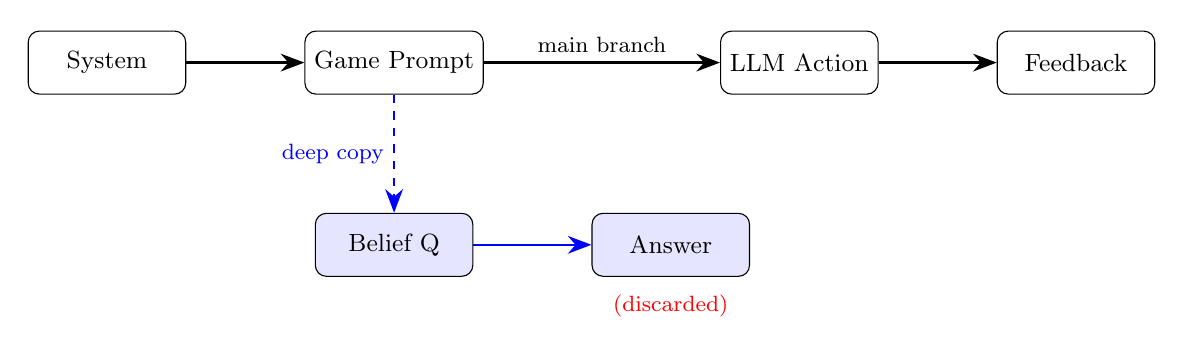
\begin{tikzpicture}[
    node distance=1.5cm,
    box/.style={rectangle, draw, rounded corners, minimum height=0.8cm, minimum width=2cm, font=\small},
    arrow/.style={-{Stealth[length=3mm]}, thick}
]
    % Main branch
    \node[box] (sys) {System};
    \node[box, right=of sys] (prompt) {Game Prompt};
    \node[box, right=3cm of prompt] (action) {LLM Action};
    \node[box, right=of action] (feedback) {Feedback};

    \draw[arrow] (sys) -- (prompt);
    \draw[arrow] (prompt) -- node[above, font=\footnotesize] {main branch} (action);
    \draw[arrow] (action) -- (feedback);

    % Fork
    \node[box, below=1.5cm of prompt, fill=blue!10] (bq1) {Belief Q};
    \node[box, right=of bq1, fill=blue!10] (ba1) {Answer};
    \node[font=\footnotesize, below=0.1cm of ba1, text=red] {(discarded)};

    \draw[arrow, dashed, blue] (prompt.south) -- node[left, font=\footnotesize, text=blue] {deep copy} (bq1);
    \draw[arrow, blue] (bq1) -- (ba1);
\end{tikzpicture}
\caption{Fork-and-elicit architecture. Beliefs are elicited in a deep-copied conversation branch \emph{before} the LLM responds with its action. The branch is discarded after extraction.}
\label{fig:fork}
\end{figure}

The protocol proceeds as follows:
\begin{enumerate}[nosep]
    \item The game prompt is appended to the conversation (main branch).
    \item The conversation is deep-copied to create an isolated belief branch.
    \item Belief questions (with optional PSR framing) are asked in the branch.
    \item Beliefs are extracted from the branch responses via regex-based parsing.
    \item The branch is discarded; the main conversation never sees the belief questions.
    \item The LLM responds with its action in the main branch.
\end{enumerate}

This design ensures: (a)~beliefs are \emph{pre-decision} (enabling causal identification of the belief$\to$action relationship), and (b)~the game conversation is never contaminated by belief elicitation (no experimenter demand effects within the game).


\subsection{Games and Strategic Rationale}
\label{sec:games}

We select five games where beliefs have genuine strategic relevance---none has a dominant strategy equilibrium (in the relevant setting).

\begin{table}[h]
\centering
\caption{Summary of games and their belief-dependent structure.}
\label{tab:games}
\begin{tabular}{@{}lllll@{}}
\toprule
Game & Type & Action Space & Belief & Threshold \\
\midrule
Stag Hunt & Normal form & $\{\text{Stag}, \text{Hare}\}$ & $p = \Prob(\text{partner: Stag})$ & $p^* = 2/3$ \\
PD (infinite) & Repeated & $\{\text{Push}, \text{Pull}\}$ & $p = \Prob(\text{coop type})$ & $p^*(\delta)$ \\
Beauty Contest & Normal form & $[0, 100]$ & $\mu = \E[\text{others' avg}]$ & $c^* = 4\mu/7$ \\
Auction & Bayesian & $[0, v]$ & $\E[\text{opp bid}]$ & $b^* = v/2$ \\
Ultimatum & Extensive form & $[0, 100]$ & $\pi(x) = \Prob(\text{acc} \mid x)$ & FOC~\eqref{eq:ultimatum_foc} \\
\bottomrule
\end{tabular}
\end{table}


\subsection{Opponent Strategy System}
\label{sec:opponents}

For repeated games (PD, Stag Hunt), the simulated opponent follows a configurable strategy:
\begin{itemize}[nosep]
    \item \texttt{RANDOM($p$)}: cooperates with probability $p$ each round (i.i.d.).
    \item \texttt{TIT\_FOR\_TAT}: cooperates in round 1, then mirrors the player's previous action.
    \item \texttt{ALWAYS\_COOPERATE} / \texttt{ALWAYS\_DEFECT}: deterministic strategies.
    \item \texttt{CUSTOM(sequence)}: plays a pre-specified sequence of actions.
\end{itemize}

For the Beauty Contest, other players' choices are drawn from a configurable distribution (default: Uniform[0,100]). For the Auction, the opponent bids according to a configurable function (default: BNE $b = v/2$).


\subsection{Dual Elicitation: PSR vs Direct Ask}
\label{sec:dual}

Each belief question can be asked in two modes:
\begin{itemize}[nosep]
    \item \textbf{Incentivized (PSR)}: Includes an explanation of the quadratic scoring rule and frames the question as incentive-compatible.
    \item \textbf{Direct ask}: Simply asks for the probability or expectation without scoring-rule framing.
\end{itemize}

This is controlled by the \texttt{incentivized} parameter in the game configuration.


% =====================================================================
\section{Experiment 1: Belief-Action Consistency}
\label{sec:exp1}
% =====================================================================

\subsection{Research Question}

\begin{quote}
\emph{Are LLM-elicited beliefs consistent with observed actions under expected utility maximization or quantal response equilibrium?}
\end{quote}

This experiment is \textbf{observational}: we measure beliefs and actions in normal gameplay without manipulation. It establishes that beliefs are (i)~measurable and (ii)~predictive.

\subsection{Design}

\begin{table}[h]
\centering
\caption{Experiment 1 design matrix.}
\label{tab:exp1}
\begin{tabular}{@{}lcccl@{}}
\toprule
Game & $N$ & Rounds & Opponent & Primary Test \\
\midrule
Stag Hunt & 50 & 5 & RANDOM(0.5) & Threshold at $p = 2/3$ \\
PD (infinite) & 50 & 10+ & RANDOM(0.5) & Threshold under restricted types \\
Beauty Contest & 50 & 3 & Uniform random & $c \approx 4\mu/7$ \\
Auction & 50 & 1 (per instance) & BNE ($v/2$) & Bid-belief regression \\
Ultimatum & 50 & 1 (per instance) & --- & Offer $= \argmax V(x, \pi)$ \\
\bottomrule
\end{tabular}
\end{table}

For each instance, we record the tuple $(b_i, a_i)$ where $b_i$ is the elicited belief and $a_i$ is the observed action. In multi-round games, we collect one tuple per round.

\textbf{PD framing}: The prompt states ``you will play for many rounds'' without specifying a total, approximating an infinite horizon. The belief question asks about $\Prob(\text{opponent is cooperative type})$.


\subsection{Game-Specific Analysis Plans}

\paragraph{Stag Hunt (primary test).}
\begin{enumerate}[nosep]
    \item \textbf{BACR}: Compute the Belief-Action Consistency Rate = fraction of observations where $a_i$ matches $\argmax_a V(a, b_i)$. Under EU: Stag if $b_i > 2/3$, else Hare.
    \item \textbf{Logistic regression}: Fit $\text{logit}(\Prob(\text{Stag})) = \beta_0 + \beta_1 \cdot b_i$. The estimated threshold is $\hat{p}^* = -\beta_0/\beta_1$. Under EU: $\hat{p}^* \approx 2/3$.
    \item \textbf{QRE estimation}: Estimate $\hat\lambda$ from~\eqref{eq:logistic_sh} via maximum likelihood. Test $H_0: \lambda = 0$ (random choice) vs.\ $H_1: \lambda > 0$.
    \item \textbf{Binned analysis}: Partition beliefs into $[0, 1/3)$, $[1/3, 2/3)$, $[2/3, 1]$. Plot fraction choosing Stag in each bin. Expect: low, mixed, high.
\end{enumerate}

\paragraph{PD (infinite, restricted types).}
\begin{enumerate}[nosep]
    \item Correlation between $\Prob(\text{cooperative type})$ and Push choice.
    \item Round-by-round Bayesian updating: does $b_{i,r+1}$ increase after observing opponent Push and decrease after Pull?
    \item Test whether cooperation rate tracks the theoretically predicted threshold $p^*(\delta)$.
\end{enumerate}

\paragraph{Beauty Contest.}
\begin{enumerate}[nosep]
    \item Regression: $c_i = \alpha + \beta \cdot \mu_i + \epsilon_i$. Theory predicts $\alpha \approx 0$, $\beta \approx 4/7$.
    \item Level-$k$ classification: cluster $\mu_i$ values and match to the geometric sequence $50 \cdot (4/7)^{k-1}$.
    \item Within-level consistency: conditional on $\mu_i$, is $c_i$ close to the best response $4\mu_i/7$?
\end{enumerate}

\paragraph{Auction.}
\begin{enumerate}[nosep]
    \item Regression: $b_i = \alpha + \beta_1 v_i + \beta_2 \E_i[\text{opp bid}] + \epsilon_i$. Theory: $\beta_1 \approx 0.5$.
    \item Bid shading: compute $b_i / v_i$ and compare to theoretical $0.5$.
\end{enumerate}

\paragraph{Ultimatum.}
\begin{enumerate}[nosep]
    \item From elicited $\{\pi(10), \pi(20), \ldots, \pi(50)\}$, compute $V(x) = (100-x)\pi(x)$ for each $x$.
    \item Find $x^* = \argmax_x V(x)$ for each instance.
    \item Test: is actual offer close to $x^*$? Report correlation and mean absolute deviation.
\end{enumerate}

\subsection{Statistical Tests}

\begin{itemize}[nosep]
    \item \textbf{BACR significance}: One-sample proportion test, $H_0: \text{BACR} = 0.5$ (chance), $H_1: \text{BACR} > 0.5$.
    \item \textbf{Logistic coefficient}: Wald test for $\beta_1 > 0$.
    \item \textbf{QRE}: Likelihood ratio test, $\lambda = 0$ vs.\ $\lambda > 0$.
    \item \textbf{Regressions}: OLS with robust standard errors; report $R^2$.
\end{itemize}


% =====================================================================
\section{Experiment 2: Causal Intervention}
\label{sec:exp2}
% =====================================================================

\subsection{Research Question}

\begin{quote}
\emph{Does exogenously manipulating beliefs causally change the LLM's strategy?}
\end{quote}

Experiment~1 establishes correlation. Experiment~2 tests causation via three distinct manipulation channels. The cross-experiment comparison provides a triangulation argument.


\subsection{Experiment 2A: Information Treatment}
\label{sec:exp2a}

\paragraph{Rationale.}
We provide the LLM with exogenous information about the opponent's past behavior. This is analogous to the ``partner history'' treatment in human experiments \citep{charness2006intentions}. The information should shift beliefs, which should in turn shift actions.

\paragraph{Design.}
\begin{itemize}[nosep]
    \item \textbf{Games}: Stag Hunt (5 rounds) and PD (infinite framing, 10 rounds).
    \item \textbf{Treatment variable}: $X \in \{1, 3, 5, 7, 9\}$ = number of cooperative plays out of 10 recent games described.
    \item \textbf{Per condition}: $N = 30$ instances.
    \item \textbf{Total}: $5 \times 30 \times 2 = 300$ sessions.
    \item \textbf{Prompt modification}: Before the game begins, the LLM is told: ``In this partner's 10 most recent games with other players, they chose [Stag/Push] in $X$ out of 10 games.''
    \item \textbf{Measures}: Elicited belief $b_i$ (pre-decision, in fork) and action $a_i$.
\end{itemize}

\paragraph{Analysis.}
\begin{enumerate}[nosep]
    \item \textbf{First stage}: $b_i = \gamma_0 + \gamma_1 X + \epsilon_i$. Test $\gamma_1 > 0$ (information shifts beliefs).
    \item \textbf{Reduced form}: $a_i = \delta_0 + \delta_1 X + u_i$. Test $\delta_1 > 0$ (treatment shifts actions).
    \item \textbf{Mediation / IV}: Use $X$ as an instrument for $b_i$ in the action equation:
    \begin{equation}
        a_i = \alpha + \beta \cdot b_i + \nu_i, \quad \text{instrumented by } X.
    \end{equation}
    Test for full mediation: the direct effect of $X$ on $a$ (controlling for $b$) should be zero.
    \item \textbf{Dose-response}: For Stag Hunt, the action should switch from Hare to Stag around $X = 7$ (since $p \approx X/10$ and threshold is $2/3 \approx 6.7/10$).
\end{enumerate}

\paragraph{Identification.}
Under the assumption that $X$ affects $a$ only through $b$ (exclusion restriction), the IV estimate $\hat\beta_{\text{IV}} = \hat\delta_1 / \hat\gamma_1$ identifies the causal effect of belief on action.


\subsection{Experiment 2B: Direct Belief Injection}
\label{sec:exp2b}

\paragraph{Rationale.}
The strongest test: directly state a belief and observe whether the action is consistent with EU maximization at that belief. This bypasses the belief formation process entirely.

\paragraph{Design.}
\begin{itemize}[nosep]
    \item \textbf{Games}: Stag Hunt and PD (round 1 only).
    \item \textbf{Treatment}: Injected belief $X \in \{10, 30, 50, 70, 90\}$ (\%).
    \item \textbf{Per condition}: $N = 30$.
    \item \textbf{Total}: $5 \times 30 \times 2 = 300$ sessions.
    \item \textbf{Prompt}: Standard game description + ``For this round, suppose you believe there is a $[X]\%$ chance the other player will choose [Stag/Push].''
    \item \textbf{No belief elicitation}: belief is set by design.
\end{itemize}

\paragraph{Control for instruction-following.}
A critical concern: the LLM may simply ``cooperate when told high belief'' regardless of the game structure. To control for this, we include a \textbf{modified Stag Hunt} with payoffs $(S,S)=3, (S,H)=0, (H,S)=2, (H,H)=2$, which gives threshold $p^* = 2/(3-2) \cdot (2/3) = 2$... We use payoffs where the threshold shifts to $p^* = 1/2$: specifically $(S,S)=4, (S,H)=0, (H,S)=2, (H,H)=2$, giving $V(S) = 4p$, $V(H) = 2$, threshold $p^* = 1/2$.

If the switching point moves from $2/3$ to $1/2$ when the payoffs change, this is evidence of genuine payoff-sensitive reasoning, not mere instruction-following.

\paragraph{Analysis.}
\begin{enumerate}[nosep]
    \item Plot $\Prob(\text{Stag} \mid X)$ as a function of $X$. Under EU: step function at $X = 67$. Under QRE: smooth sigmoid.
    \item Logistic fit: $\text{logit}(\Prob(\text{Stag})) = \beta_0 + \beta_1 X$. Threshold $= -\beta_0 / \beta_1$.
    \item Compare thresholds across payoff variants: $\hat{p}^*_{\text{original}} \approx 2/3$ vs.\ $\hat{p}^*_{\text{modified}} \approx 1/2$.
\end{enumerate}


\subsection{Experiment 2C: Fake History Priming}
\label{sec:exp2c}

\paragraph{Rationale.}
This is the most ecologically valid causal test. Instead of stating information or injecting beliefs, we construct a fabricated game history. The LLM must \emph{infer} beliefs from experience, then act on those beliefs. This tests the full belief formation $\to$ action pipeline.

\paragraph{Design.}
\begin{itemize}[nosep]
    \item \textbf{Game}: Stag Hunt.
    \item \textbf{Treatment}: Fabricated 5-round history where the opponent cooperated (Stag) in $k \in \{0, 1, 2, 3, 4, 5\}$ out of 5 rounds.
    \item \textbf{Per condition}: $N = 30$.
    \item \textbf{Total}: $6 \times 30 = 180$ sessions.
    \item \textbf{Implementation}: Construct a message list simulating 5 completed rounds (with alternating user/assistant messages), then present round 6.
    \item \textbf{Measures}: Elicited belief $b_6$ at round 6 (in fork) and action $a_6$.
\end{itemize}

\paragraph{Analysis.}
\begin{enumerate}[nosep]
    \item \textbf{Belief tracking}: Does $b_6$ increase monotonically with $k/5$?
    \item \textbf{Belief-action consistency}: Does the $b_6 \to a_6$ mapping match the observational relationship from Experiment~1?
    \item \textbf{Slope comparison}: Estimate $\beta_{\text{Exp1}}$ (observational) and $\beta_{\text{Exp2C}}$ (priming). If $\beta_{\text{Exp1}} \approx \beta_{\text{Exp2C}}$, the same causal mechanism operates in both settings.
\end{enumerate}


\subsection{Cross-Experiment Causal Identification}
\label{sec:cross_exp}

The three sub-experiments provide a \emph{triangulation} of the causal claim. Table~\ref{tab:triangulation} summarizes the diagnostic logic.

\begin{table}[h]
\centering
\caption{Diagnostic interpretation of sub-experiment results.}
\label{tab:triangulation}
\begin{tabular}{@{}cccp{6cm}@{}}
\toprule
2A & 2B & 2C & Interpretation \\
\midrule
\checkmark & \checkmark & \checkmark & \textbf{Strong evidence}: Belief is a genuine causal mediator. It responds to information, is used for payoff-sensitive reasoning, and is formed from experience. \\
$\times$ & \checkmark & $\times$ & Instruction-following: LLM complies with stated beliefs but does not form or use beliefs from context. \\
\checkmark & $\times$ & \checkmark & Contextual reasoning: LLM forms beliefs from context but ignores explicit belief statements. \\
$\times$ & $\times$ & $\times$ & No causal role: beliefs and actions are jointly determined by prompts without beliefs mediating. \\
\bottomrule
\end{tabular}
\end{table}


% =====================================================================
\section{Experiment 3: Elicitation Methodology Comparison}
\label{sec:exp3}
% =====================================================================

\subsection{Research Question}

\begin{quote}
\emph{Does PSR framing change LLM belief reports compared to direct ask, and if so, which method produces more reliable and predictive beliefs?}
\end{quote}

\subsection{Design}

\begin{itemize}[nosep]
    \item \textbf{Between-subject}: Each instance is assigned to either PSR or direct ask.
    \item \textbf{Games}: All five.
    \item \textbf{Per condition per game}: $N = 50$.
    \item \textbf{Total}: $2 \times 5 \times 50 = 500$ sessions.
    \item \textbf{Opponent strategies}: Identical across conditions.
\end{itemize}

\subsection{Measures and Analysis}

\begin{enumerate}[nosep]
    \item \textbf{Mean belief}: Two-sample $t$-test or Wilcoxon rank-sum. Does PSR shift average reported beliefs?
    \item \textbf{Belief variance}: Levene's test. Does PSR reduce extreme beliefs?
    \item \textbf{Calibration}: For games with known opponent strategy (e.g., RANDOM(0.5) in Stag Hunt), compare $|\E[b_i] - 0.5|$ across conditions.
    \item \textbf{Predictive power}: Regress $a_i$ on $b_i$ separately for each condition. Compare $R^2$ and coefficient magnitudes.
    \item \textbf{Extraction success}: Compare null-extraction rates (fraction of responses where belief parsing fails).
\end{enumerate}

This experiment provides practical recommendations for researchers: which elicitation mode to use when studying LLM beliefs.


% =====================================================================
\section{Preliminary Results}
\label{sec:results}
% =====================================================================

We report results from an initial run using \texttt{gpt-4.1-mini} via a compatible API endpoint. Unless otherwise stated, all beliefs are elicited in PSR (incentivized) mode.

\subsection{Experiment 1: Belief-Action Consistency}

\subsubsection{Stag Hunt ($N=50$, 5 rounds, RANDOM(0.5) opponent)}

Across 250 round-level observations:

\begin{itemize}[nosep]
    \item \textbf{BACR} (EU threshold $p^*=2/3$): $0.596$ ($149/250$).
    \item \textbf{Logistic regression}: $\text{logit}(\Prob(\text{Stag})) = \hat\beta_0 + 8.312 \cdot b_i$ ($p < 0.0001$). Estimated threshold $\hat{p}^* = 0.348$, well below the EU-predicted $2/3$, indicating that the LLM cooperates more readily than strict EU predicts---consistent with a QRE model with moderate $\lambda$.
    \item \textbf{Calibration}: Mean elicited belief $= 0.488$ vs.\ true opponent cooperation rate $0.5$; bias $= -0.012$. Beliefs are well-calibrated.
    \item \textbf{Binned analysis}:
\end{itemize}

\begin{center}
\begin{tabular}{@{}lcc@{}}
\toprule
Belief bin & Fraction choosing Stag & $n$ \\
\midrule
$[0.00, 0.33)$ & 0.38 & 93 \\
$[0.33, 0.67)$ & 0.71 & 91 \\
$[0.67, 1.00]$ & 0.98 & 66 \\
\bottomrule
\end{tabular}
\end{center}

The monotonically increasing pattern is strong: at low beliefs, Stag is rare; at high beliefs, it is near-universal.

\subsubsection{Prisoner's Dilemma ($N=50$, 10 rounds, $\delta=0.9$, RANDOM(0.5) opponent)}

Across 484 valid round-level observations (dual beliefs: type + action per round):

\begin{itemize}[nosep]
    \item \textbf{BACR (type belief)}: $0.444$ ($215/484$). Lower than Stag Hunt, partly because $\delta=0.9 > 3/4$ makes cooperation optimal for any $p>0$ against TFT, so the threshold is not as discriminating.
    \item \textbf{Bayesian updating}: After observing opponent Push, the mean change in $\Prob(\text{cooperative type})$ is $+0.200$ ($n=192$). After opponent Pull, the mean change is $-0.152$ ($n=228$). Both directions are correct and substantial, confirming that the LLM updates beliefs in the Bayesian direction.
\end{itemize}

\subsubsection{Beauty Contest ($N=50$, 3 rounds, $p=2/3$, 3 players)}

Across 150 round-level observations:

\begin{itemize}[nosep]
    \item \textbf{Regression}: $c_i = 4.10 + 0.704 \cdot \mu_i$. Theory predicts $c = 0 + 0.571\mu$. The estimated slope $\hat\beta = 0.704$ is above the best-response coefficient $4/7 \approx 0.571$, but the direction and magnitude are consistent.
    \item \textbf{$R^2 = 0.521$}: Beliefs explain over half the variance in chosen numbers.
    \item \textbf{Level-$k$ distribution}: $L_1$: 89, $L_2$: 54, $L_3$: 5, $L_4$: 2. The model predominantly operates at levels 1--2, consistent with findings in human experiments \citep{nagel1995unraveling}.
    \item \textbf{Best-response MAD}: $10.32$ (mean absolute deviation from $c^*(\mu_i) = 4\mu_i/7$).
\end{itemize}

\subsubsection{First-Price Auction ($N=50$, BNE opponent)}

\begin{itemize}[nosep]
    \item \textbf{Bid regression}: $\text{bid}_i = -0.57 + 0.558 \cdot v_i + 0.009 \cdot \E_i[\text{opp bid}]$. The coefficient on valuation ($\hat\beta_v = 0.558$) is close to the BNE prediction of $0.5$.
    \item \textbf{Bid shading}: Mean $\text{bid}/\text{valuation} = 0.550$, close to the theoretical $0.5$.
    \item The near-zero coefficient on $\E[\text{opp bid}]$ ($0.009$) suggests the model primarily anchors on its own valuation, as theory predicts.
\end{itemize}

\subsubsection{Ultimatum Game ($N=50$, Proposer)}

\begin{itemize}[nosep]
    \item \textbf{Actual offers}: mean $= \$30.4$, std $= \$2.0$. Offers are tightly clustered.
    \item \textbf{Optimal offers} (computed from each instance's elicited acceptance schedule): mean $= \$23.6$.
    \item \textbf{Consistency}: MAD $= \$6.8$, exact match rate $= 34\%$, correlation $= 0.060$.
    \item \textbf{Mean acceptance schedule}: $\pi(10)=0.533$, $\pi(20)=0.800$, $\pi(30)=0.927$, $\pi(40)=0.973$, $\pi(50)=0.990$.
    \item The model over-offers relative to its own beliefs (offers $\$30$ on average when beliefs imply $\$24$ is optimal), suggesting a ``fairness'' bias similar to human proposers \citep{guth1982experimental}.
\end{itemize}

\subsubsection{Summary}

\begin{table}[h]
\centering
\caption{Experiment 1 summary: belief-action consistency across five games (\texttt{gpt-4.1-mini}, $N=50$).}
\label{tab:exp1_results}
\begin{tabular}{@{}llll@{}}
\toprule
Game & Primary metric & Result & Theory \\
\midrule
Stag Hunt & BACR & 0.596 & $>0.5$ \\
Stag Hunt & Logistic $\hat\beta_1$ & 8.312 ($p<0.0001$) & $>0$ \\
Stag Hunt & Calibration bias & $-0.012$ & $\approx 0$ \\
PD (infinite) & Bayesian update $\Delta b$ after Push & $+0.200$ & $>0$ \\
PD (infinite) & Bayesian update $\Delta b$ after Pull & $-0.152$ & $<0$ \\
Beauty Contest & $\hat\beta$ (choice on belief) & 0.704 & 0.571 \\
Beauty Contest & $R^2$ & 0.521 & --- \\
Auction & $\hat\beta_v$ (bid on valuation) & 0.558 & 0.500 \\
Ultimatum & Offer MAD from optimal & \$6.8 & \$0 \\
\bottomrule
\end{tabular}
\end{table}


\subsection{Experiment 2: Causal Intervention}

\subsubsection{Experiment 2A: Information Treatment ($N=30$ per condition)}

\paragraph{Stag Hunt} ($N_{\text{total}}=149$ valid observations across 5 treatments).

\begin{itemize}[nosep]
    \item \textbf{First stage}: $b_i = -0.000 + 0.100 \cdot X$ ($R^2 = 1.000$, $p < 0.0001$). Beliefs track the treatment essentially perfectly: the model reports $b \approx X/10$.
    \item \textbf{Reduced form}: $a_i = 0.075 + 0.123 \cdot X$ ($R^2 = 0.574$, $p < 0.0001$). The treatment causally shifts actions.
    \item \textbf{IV estimate}: $\hat\beta_{\text{IV}} = 0.123 / 0.100 = 1.233$, the estimated causal effect of a 1-unit increase in $b$ on cooperation probability.
\end{itemize}

\begin{center}
\begin{tabular}{@{}cccc@{}}
\toprule
Treatment $X$ & Mean belief $\hat{b}$ & $\Prob(\text{Stag})$ & $n$ \\
\midrule
1 & 0.100 & 0.00 & 30 \\
3 & 0.300 & 0.53 & 30 \\
5 & 0.500 & 0.93 & 29 \\
7 & 0.700 & 1.00 & 30 \\
9 & 0.900 & 1.00 & 30 \\
\bottomrule
\end{tabular}
\end{center}

The dose-response pattern is striking: cooperation jumps from 0\% at $X=1$ to 93\% at $X=5$, saturating at 100\% by $X=7$. This is consistent with a switching threshold around $X \approx 3\text{--}5$, or $b \approx 0.3\text{--}0.5$, matching the Experiment~1 logistic threshold of $\hat{p}^*=0.348$.

\paragraph{Prisoner's Dilemma} ($N_{\text{total}}=147$).

\begin{itemize}[nosep]
    \item \textbf{First stage}: $b_i = 0.003 + 0.100 \cdot X$ ($R^2 = 0.997$, $p < 0.0001$). Near-perfect belief tracking.
    \item \textbf{Reduced form}: $a_i = -0.164 + 0.079 \cdot X$ ($R^2 = 0.278$, $p < 0.0001$). Significant but weaker causal effect on actions.
    \item \textbf{IV estimate}: $\hat\beta_{\text{IV}} = 0.788$.
\end{itemize}

\begin{center}
\begin{tabular}{@{}cccc@{}}
\toprule
Treatment $X$ & Mean belief $\hat{b}$ & $\Prob(\text{Push})$ & $n$ \\
\midrule
1 & 0.103 & 0.00 & 29 \\
3 & 0.300 & 0.03 & 29 \\
5 & 0.505 & 0.14 & 29 \\
7 & 0.700 & 0.33 & 30 \\
9 & 0.900 & 0.63 & 30 \\
\bottomrule
\end{tabular}
\end{center}

Cooperation increases monotonically with treatment intensity but more gradually than in Stag Hunt, consistent with the PD's stronger temptation to defect. Even at $X=9$ (90\% belief in cooperative type), only 63\% cooperate---suggesting the LLM applies additional discounting beyond pure EU.


\subsubsection{Experiment 2B: Direct Belief Injection ($N=30$ per condition)}

\paragraph{Standard Stag Hunt (threshold $p^*=2/3$).}

\begin{center}
\begin{tabular}{@{}ccc@{}}
\toprule
Injected belief $X\%$ & $\Prob(\text{Stag})$ & $n$ \\
\midrule
10 & 0.00 & 30 \\
30 & 0.00 & 30 \\
50 & 0.00 & 30 \\
70 & 1.00 & 30 \\
90 & 1.00 & 30 \\
\bottomrule
\end{tabular}
\end{center}

The action profile is a near-perfect step function: 0\% Stag at $X \leq 50\%$, 100\% Stag at $X \geq 70\%$. The logistic regression yields $\hat{p}^* = 59.7\%$, consistent with the theoretical $p^* = 66.7\%$.

\paragraph{Modified Stag Hunt (threshold $p^*=1/2$).}

\begin{center}
\begin{tabular}{@{}ccc@{}}
\toprule
Injected belief $X\%$ & $\Prob(\text{Stag})$ & $n$ \\
\midrule
10 & 0.00 & 30 \\
30 & 0.00 & 30 \\
50 & 0.33 & 30 \\
70 & 1.00 & 30 \\
90 & 1.00 & 30 \\
\bottomrule
\end{tabular}
\end{center}

The switching point moves left: at $X=50\%$, 33\% now choose Stag (vs.\ 0\% in the standard variant). The logistic threshold is $\hat{p}^* = 50.5\%$, closely matching the modified game's theoretical $p^* = 50\%$. \textbf{The threshold shift from $59.7\%$ to $50.5\%$ when payoffs change confirms payoff-sensitive reasoning, ruling out mere instruction-following.}

\paragraph{Prisoner's Dilemma (repeated-game framing).}

\begin{center}
\begin{tabular}{@{}ccc@{}}
\toprule
Injected belief $X\%$ & $\Prob(\text{Push})$ & $n$ \\
\midrule
10 & 0.03 & 30 \\
30 & 0.07 & 30 \\
50 & 0.27 & 30 \\
70 & 0.23 & 30 \\
90 & 0.77 & 30 \\
\bottomrule
\end{tabular}
\end{center}

Cooperation increases from 3\% to 77\%, with estimated threshold $\hat{p}^* = 76.8\%$. The gradual increase (rather than a sharp step) is consistent with a QRE model with lower $\lambda$ than in Stag Hunt.


\subsubsection{Experiment 2C: Fake History Priming ($N=30$ per condition)}

\begin{center}
\begin{tabular}{@{}cccc@{}}
\toprule
$k$ (Stag in history) & Mean belief $\hat{b}_6$ & Std & $\Prob(\text{Stag at round 6})$ \\
\midrule
0 & 0.063 & 0.046 & 0.00 \\
1 & 0.338 & 0.219 & 0.27 \\
2 & 0.433 & 0.153 & 0.33 \\
3 & 0.595 & 0.099 & 0.70 \\
4 & 0.769 & 0.112 & 0.83 \\
5 & 0.903 & 0.012 & 1.00 \\
\bottomrule
\end{tabular}
\end{center}

\begin{itemize}[nosep]
    \item \textbf{Belief tracking}: Beliefs increase \emph{monotonically} with $k$ ($0.063 \to 0.903$). Regression: $b_6 = \alpha + 0.162 \cdot k$ ($R^2 = 0.816$, $p < 0.0001$).
    \item \textbf{Action tracking}: Stag rate increases monotonically ($0\% \to 100\%$).
    \item \textbf{Belief$\to$action logistic}: $\hat\beta_1 = 11.73$, threshold $= 0.519$. This is comparable to the observational threshold from Experiment~1 ($\hat{p}^* = 0.348$, $\hat\beta_1 = 8.31$), and both are below the EU-predicted $2/3$. The similarity of the logistic slopes across observational (Exp~1) and experimental (Exp~2C) data supports the conclusion that the \textbf{same belief$\to$action mechanism operates in both settings}.
\end{itemize}


\subsubsection{Cross-Experiment Summary}

Applying the diagnostic logic from Table~\ref{tab:triangulation}:

\begin{center}
\begin{tabular}{@{}ccl@{}}
\toprule
Sub-experiment & Outcome & Evidence \\
\midrule
2A (Info treatment) & \checkmark & Beliefs track treatment perfectly; actions shift causally \\
2B (Direct injection) & \checkmark & Threshold shifts with payoffs (59.7\% $\to$ 50.5\%) \\
2C (Fake history) & \checkmark & Beliefs formed from experience; same $b\to a$ mechanism \\
\bottomrule
\end{tabular}
\end{center}

All three channels confirm belief as a causal mediator: $\checkmark$/$\checkmark$/$\checkmark$ corresponds to \textbf{``Strong evidence''} in Table~\ref{tab:triangulation}. Belief responds to information (2A), is used for payoff-sensitive reasoning (2B), and is formed from experience (2C).


% =====================================================================
\section{Power Analysis and Experimental Budget}
\label{sec:power}
% =====================================================================

\begin{table}[h]
\centering
\caption{Power analysis for key tests.}
\label{tab:power}
\begin{tabular}{@{}llccl@{}}
\toprule
Experiment & Test & $N_{\text{obs}}$ & Power & Effect size \\
\midrule
1 (Stag Hunt) & BACR $> 0.5$ & 250 (50$\times$5) & $> 0.99$ & 80\% vs 50\% accuracy \\
1 (Beauty) & $\beta = 4/7$ & 150 (50$\times$3) & $> 0.95$ & $R^2 > 0.3$ \\
2A (Info) & Linear trend $\gamma_1$ & 150 (30$\times$5) & $> 0.90$ & $r = 0.3$ \\
2B (Injection) & Logistic threshold & 150 (30$\times$5) & $> 0.95$ & OR $= 3$ per 20pp \\
2C (Priming) & Slope comparison & 180 (30$\times$6) & $> 0.85$ & $|\Delta\beta| / \text{SE} > 2$ \\
3 (PSR vs Direct) & Mean diff & 100 (50$\times$2) & $> 0.80$ & Cohen's $d = 0.57$ \\
\bottomrule
\end{tabular}
\end{table}

\paragraph{Total experimental budget.}
\begin{itemize}[nosep]
    \item Experiment 1: $50 \times 5 = 250$ sessions
    \item Experiment 2A: $5 \times 30 \times 2 = 300$ sessions
    \item Experiment 2B: $5 \times 30 \times 2 + $ control variant $= 300 + 150 = 450$ sessions
    \item Experiment 2C: $6 \times 30 = 180$ sessions
    \item Experiment 3: $2 \times 5 \times 50 = 500$ sessions
    \item \textbf{Total}: $\approx 1{,}680$ sessions
\end{itemize}

At approximately 10 seconds per session, total runtime is $\approx 4.7$ hours.


% =====================================================================
\section{Implementation Logic}
\label{sec:implementation}
% =====================================================================

All experiments build on the \texttt{belief\_elicitation} Python package. We describe the mapping from experimental design to code.

\subsection{Experiment 1: Observational}

Uses existing game runners directly. No new code required.

\begin{algorithmic}[1]
\STATE \textbf{Input}: game $g$, $N$ instances, opponent strategy $\sigma$, rounds $R$
\STATE runner, get\_response $\leftarrow$ create\_belief\_aware\_runner(client, model)
\STATE config $\leftarrow$ get\_config($g$, n\_rounds=$R$, incentivized=True)
\STATE records $\leftarrow$ run\_$g$\_with\_beliefs(runner, get\_response, $N$, $R$, $\sigma$, config)
\STATE \textbf{Output}: records containing beliefs $\{b_{ir}\}$ and actions $\{a_{ir}\}$
\end{algorithmic}

\subsection{Experiment 2A: Information Treatment}

Requires a wrapper function that modifies the initial game prompt.

\begin{algorithmic}[1]
\STATE \textbf{Input}: game $g$, treatment $X$, $N$ instances
\STATE info\_text $\leftarrow$ ``In this partner's 10 most recent games, they chose [coop] in $X$ out of 10.''
\STATE prompt\_modified $\leftarrow$ info\_text + standard game prompt
\STATE Run game with prompt\_modified using existing fork-and-elicit pipeline
\STATE \textbf{Output}: $(b_i, a_i, X)$ tuples
\end{algorithmic}

\textbf{Key implementation detail}: The modification is purely to the prompt text---the fork-and-elicit machinery operates identically.

\subsection{Experiment 2B: Direct Belief Injection}

\begin{algorithmic}[1]
\STATE \textbf{Input}: game $g$, injected belief $X\%$, $N$ instances
\STATE injection $\leftarrow$ ``Suppose you believe $\Prob(\text{coop}) = X\%$.''
\STATE prompt\_modified $\leftarrow$ standard game prompt + injection
\STATE Run game with prompt\_modified, belief\_config = None (skip elicitation)
\STATE \textbf{Output}: $(a_i, X)$ tuples
\end{algorithmic}

\subsection{Experiment 2C: Fake History Priming}

\begin{algorithmic}[1]
\STATE \textbf{Input}: cooperation rate $k/5$, $N$ instances
\STATE messages $\leftarrow$ construct\_fake\_history(game, $k$, 5)
\COMMENT{Build 5 rounds of fabricated play}
\STATE Append round-6 prompt to messages
\STATE Fork and elicit belief $b_6$ from messages
\STATE Get LLM action $a_6$ in main branch
\STATE \textbf{Output}: $(b_6, a_6, k)$ tuples
\end{algorithmic}

\texttt{construct\_fake\_history} builds a message list with alternating user/assistant exchanges simulating past rounds, using \texttt{OpponentStrategy(CUSTOM, custom\_sequence=[...])} to control the fabricated opponent actions.

\subsection{Experiment 3: Methodology Comparison}

Uses existing \texttt{incentivized=True/False} parameter. No new code required.

\begin{algorithmic}[1]
\FOR{mode $\in$ \{PSR, direct\}}
    \STATE config $\leftarrow$ get\_config($g$, incentivized=(mode == PSR))
    \STATE records\_mode $\leftarrow$ run\_$g$\_with\_beliefs(..., belief\_config=config)
\ENDFOR
\STATE Compare records\_PSR vs records\_direct
\end{algorithmic}


% =====================================================================
\appendix
\section{Payoff Matrices and Equilibrium Derivations}
\label{app:payoffs}
% =====================================================================

\subsection{Stag Hunt Equilibria}

The Stag Hunt has two pure-strategy Nash equilibria: (Stag, Stag) and (Hare, Hare). The mixed-strategy equilibrium has each player choosing Stag with probability $2/3$. (Stag, Stag) is \emph{payoff-dominant} (both get 4 vs.\ both get 2), while (Hare, Hare) is \emph{risk-dominant} (Hare guarantees at least 2, while Stag risks 0).

\subsection{PD Cooperation Threshold Derivation}

Consider the infinitely repeated PD with discount factor $\delta$ and type space $\Theta = \{\text{TFT}, \text{selfish}\}$. Let $p = \Prob(\text{TFT})$.

Against TFT, always cooperating yields:
\[
V_{\text{coop}}^{\text{TFT}} = \sum_{t=0}^{\infty} \delta^t \cdot 400 = \frac{400}{1-\delta}.
\]

Deviating to Pull in round 1 against TFT yields 700 in round 1, then TFT retaliates:
\[
V_{\text{deviate}}^{\text{TFT}} = 700 + \sum_{t=1}^{\infty} \delta^t \cdot 300 = 700 + \frac{300\delta}{1-\delta}.
\]

Against selfish type, the payoff is $\frac{300}{1-\delta}$ regardless.

Cooperation is optimal when:
\[
p \cdot \frac{400}{1-\delta} + (1-p) \cdot \frac{300}{1-\delta} > p \cdot \left(700 + \frac{300\delta}{1-\delta}\right) + (1-p) \cdot \frac{300}{1-\delta}.
\]

Simplifying:
\[
p \cdot \frac{400}{1-\delta} > p \cdot 700 + p \cdot \frac{300\delta}{1-\delta}
\]
\[
\frac{400}{1-\delta} > 700 + \frac{300\delta}{1-\delta}
\]
\[
\frac{400 - 300\delta}{1-\delta} > 700
\]
\[
400 - 300\delta > 700(1-\delta) = 700 - 700\delta
\]
\[
400\delta > 300
\]
\[
\delta > \frac{3}{4}.
\]

So for $\delta > 3/4$, cooperation is optimal against TFT regardless of $p$ (as long as $p > 0$). The threshold on $p$ binds only when $\delta < 3/4$:
\[
p^* = \frac{300(1-\delta)}{400\delta - 300\delta} = \frac{300(1-\delta)}{100\delta} = \frac{3(1-\delta)}{\delta}.
\]

For this to be a valid probability ($p^* < 1$), we need $\delta > 3/4$.

\subsection{Beauty Contest Level-$k$ Sequence}

For $n = 3$ players and $p = 2/3$, best response to belief $\mu$ is $c^*(\mu) = 4\mu/7$:

\begin{center}
\begin{tabular}{@{}ccc@{}}
\toprule
Level $k$ & Belief $\mu_k$ & Choice $c_k = 4\mu_k/7$ \\
\midrule
1 & 50.00 & 28.57 \\
2 & 28.57 & 16.33 \\
3 & 16.33 & 9.33 \\
4 & 9.33 & 5.33 \\
$\infty$ & 0 & 0 \\
\bottomrule
\end{tabular}
\end{center}


\section{Prompt Templates}
\label{app:prompts}

\subsection{Stag Hunt --- Game Prompt (Round 1)}

\begin{quote}
\small
You're paired with another player. Each round, you both simultaneously choose either `Stag' or `Hare'. Your payoffs depend on both choices:

\begin{itemize}[nosep]
    \item Both choose `Stag': Each earns 4 points
    \item Both choose `Hare': Each earns 2 points
    \item You choose `Stag', the other chooses `Hare': You earn 0 points, the other earns 3 points
    \item You choose `Hare', the other chooses `Stag': You earn 3 points, the other earns 0 points
\end{itemize}

Which would you choose in the first round? Please highlight your choice with [] (i.e., [Stag] or [Hare]).
\end{quote}

\subsection{Belief Elicitation --- PSR Mode (Stag Hunt)}

\begin{quote}
\small
Before you make your decision, I'd like to understand your expectations about the other player's likely choice.

Your payment depends on accuracy via a quadratic scoring rule: You earn $100 - 100 \times (p_{\text{reported}} - I_{\text{realized}})^2$ points, where $I_{\text{realized}} = 1$ if the event occurs, 0 otherwise. Reporting your true belief maximizes your expected score.

What probability (0--100\%) do you assign to each of the other player's possible actions in this round?

--- Stag: \_\_\_\%\\
--- Hare: \_\_\_\%

(Must sum to 100\%. Highlight each probability, e.g., [60]\% and [40]\%)
\end{quote}

\subsection{Information Treatment (Experiment 2A)}

\begin{quote}
\small
Before the game begins, you learn that in this partner's 10 most recent games with other players, they chose `Stag' in $X$ out of 10 games.

[Standard game prompt follows]
\end{quote}

\subsection{Belief Injection (Experiment 2B)}

\begin{quote}
\small
[Standard game prompt]

For this round, suppose you believe there is a $[X]\%$ chance the other player will choose Stag.
\end{quote}


% =====================================================================
\bibliographystyle{apalike}
\bibliography{refs}
% =====================================================================

\end{document}
